\section{Localization System Evaluation}

\subsection{Experiment Setup}

To evaluate the proposed localization system, a QR code was mounted on a wall, and the user's pose relative to it was estimated using the system at different angles, distances, and lighting conditions.

\textbf{Camera Used:}\\
The rear camera of the Honor ALI-NX1 smartphone was used for all experiments.

\textbf{Camera Calibration:}\\
The camera was calibrated using our implementation. Fifteen images of a calibration pattern were taken at random angles and distances. The re-projection error was found to be 0.0737 using the mobile implantation of camera calibration explained at Section \ref{sec:camera_calibration}, demonstrating excellent calibration even with random sampling.

\textbf{QR Code Setup:}\\
The QR code was mounted on a wall at a fixed height, matching the vertical height of the mobile camera. This alignment ensured both were on the same level, reducing vertical parallax and allowing for more accurate distance estimation (see Figure~\ref{Localization-Experiment-QR-Setup}).



\begin{figure}[h!]
	\centering
	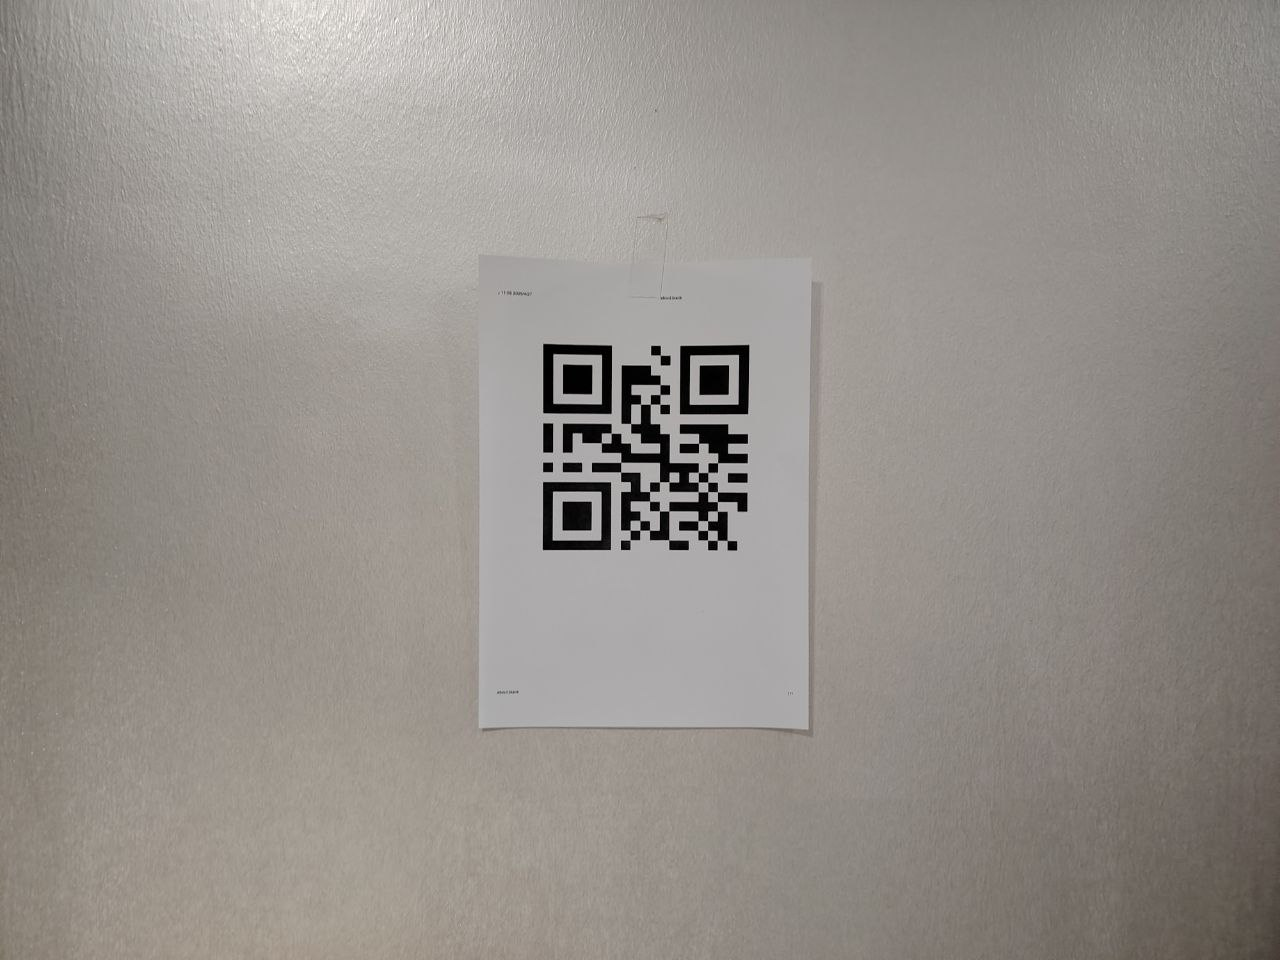
\includegraphics[width=0.7\linewidth]{assets/ch4/QR on a wall.jpg}
	\caption{A picture illustrating the QR code setup.}
	\label{Localization-Experiment-QR-Setup}
\end{figure}

\textbf{Lighting Conditions:}\\
Localization was tested under three distinct lighting conditions (see Figure~\ref{Localization-Experiment-Lighting-Conditions}):
\begin{itemize}
	\item \textbf{Perfect Lighting:} The environment is brightly lit with consistent lighting across the scanned surface. No shadows or reflections interfere with camera visibility.
	
	\item \textbf{Poor Lighting:} The environment has limited or uneven lighting, with noticeable shadows or dim areas that may partially obscure QR code visibility.
	
	\item \textbf{No Lighting at All (Dark):} The environment is completely dark or nearly so, making it impossible to see the QR code without activating the camera's built-in flash.
\end{itemize}


\begin{figure}[h!]
	\centering
	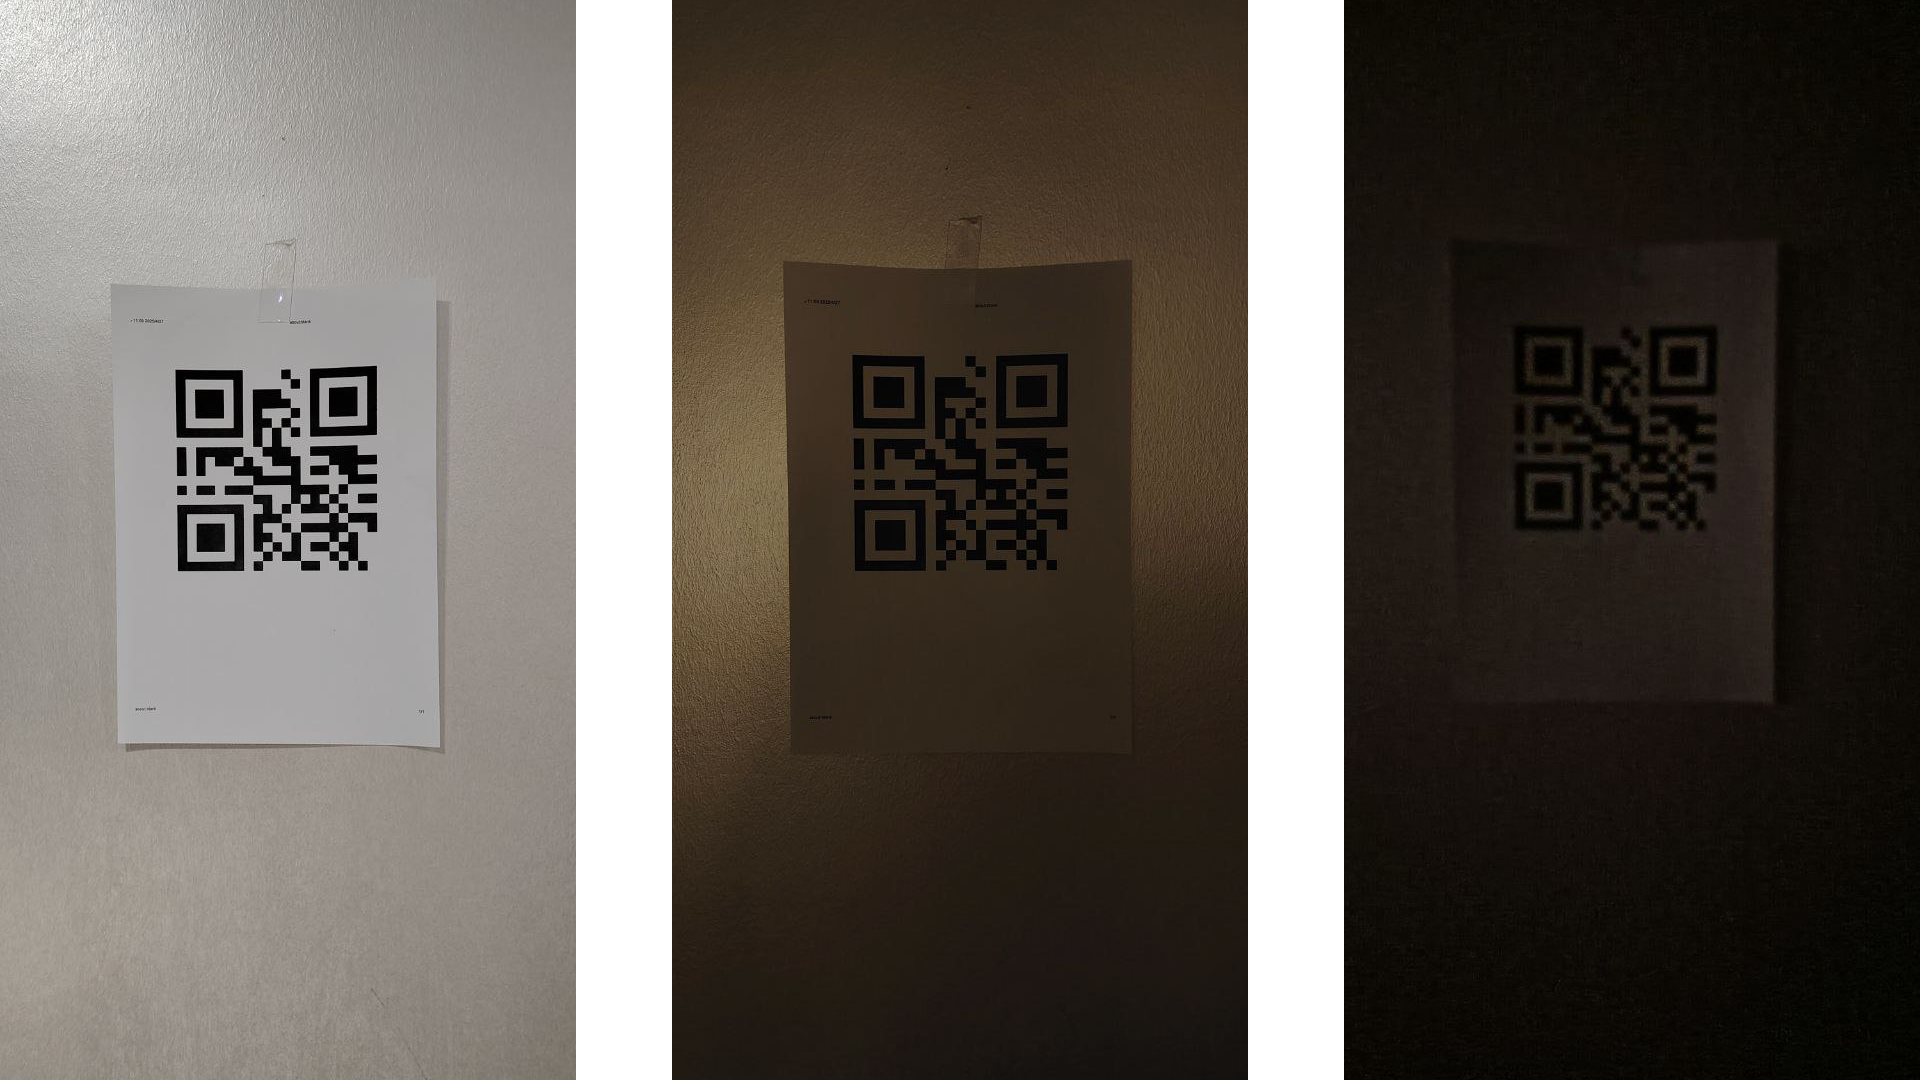
\includegraphics[width=0.7\linewidth]{assets/ch4/Three lighting conditions/Three lighting conditions.png}
	\caption{The three distinct lighting conditions: left—perfect, middle—poor, right—dark.}
	\label{Localization-Experiment-Lighting-Conditions}
\end{figure}


\subsection{Procedure}\label{sec:procedure}

The camera's $x$ and $y$ positions relative to the QR code were measured manually with an estimated accuracy of $\pm5$~mm. These measurements were used to calculate the actual distance and angle between the camera and the QR code.

For each lighting condition, the localization experiment was repeated six times. The mobile device was positioned at two distances: 1.410~m and 0.707~m. At each distance, it was placed at three different angles relative to the QR code: $0.00^\circ$, $+45.00^\circ$, and $-45.00^\circ$ as illustrated in Table \ref{table:localization_exp_res_combined}.


\subsection{Evaluation Metrics}
The evaluation metrics applied in this experiment are described in Section~\ref{sec:evaluation_metrics} of the Methodology chapter. All results and analyses in this section are based on those metrics.

\subsection{Results}

Table~\ref{table:localization_exp_res_combined} shows the results for all lighting conditions. Each row lists the estimated and actual distance and angle for a specific test case.


\begin{table}[h!]
	\caption{Estimated and real distances/angles under all lighting conditions.}
	\begin{tabularx}{0.95\textwidth} { 
			| >{\raggedright\arraybackslash}X
			| >{\centering\arraybackslash}X
			| >{\centering\arraybackslash}X
			| >{\centering\arraybackslash}X
			| >{\centering\arraybackslash}X
			| >{\centering\arraybackslash}X | }
		\hline
		Lighting & Estimated Distance & Estimated Angle & Real Distance & Real Angle \\
		\hline
		Perfect  & 0.960 m & -2.40$^\circ$  & 1.410 m & 0.00$^\circ$ \\
		Perfect  & 0.989 m & +43.20$^\circ$ & 1.410 m & +45.00$^\circ$ \\
		Perfect  & 0.981 m & -42.60$^\circ$ & 1.410 m & -45.00$^\circ$ \\
		Perfect  & 0.481 m & +3.10$^\circ$  & 0.707 m & 0.00$^\circ$ \\
		Perfect  & 0.496 m & +47.30$^\circ$ & 0.707 m & +45.00$^\circ$ \\
		Perfect  & 0.476 m & -42.60$^\circ$ & 0.707 m & -45.00$^\circ$ \\
		\hline
		Poor     & 0.984 m & -3.00$^\circ$  & 1.410 m & 0.00$^\circ$ \\
		Poor     & 0.972 m & +44.50$^\circ$ & 1.410 m & +45.00$^\circ$ \\
		Poor     & 0.946 m & -45.60$^\circ$ & 1.410 m & -45.00$^\circ$ \\
		Poor     & 0.511 m & -4.30$^\circ$  & 0.707 m & 0.00$^\circ$ \\
		Poor     & 0.485 m & +43.30$^\circ$ & 0.707 m & +45.00$^\circ$ \\
		Poor     & 0.516 m & -47.80$^\circ$ & 0.707 m & -45.00$^\circ$ \\
		\hline
		Dark     & 0.992 m & +4.20$^\circ$  & 1.410 m & 0.00$^\circ$ \\
		Dark     & 1.014 m & +44.20$^\circ$ & 1.410 m & +45.00$^\circ$ \\
		Dark     & 0.998 m & -44.80$^\circ$ & 1.410 m & -45.00$^\circ$ \\
		Dark     & 0.501 m & +3.10$^\circ$  & 0.707 m & 0.00$^\circ$ \\
		Dark     & 0.500 m & +42.70$^\circ$ & 0.707 m & +45.00$^\circ$ \\
		Dark     & 0.526 m & -48.00$^\circ$   & 0.707 m & -45.00$^\circ$ \\
		\hline
	\end{tabularx}
	\label{table:localization_exp_res_combined}
\end{table}

Evaluation results, including mean absolute error and standard deviation for each lighting condition, are presented in Table~\ref{table:localization_eval}.

\begin{table}[h!]
	\caption{Evaluation results for each lighting condition.}
	\begin{tabularx}{0.95\textwidth} { 
			| >{\raggedright\arraybackslash}X 
			| >{\centering\arraybackslash}X 
			| >{\centering\arraybackslash}X 
			| >{\centering\arraybackslash}X 
			| >{\centering\arraybackslash}X | }
		\hline
		Lighting Condition & Distance Mean Abs. Error & Angle Mean Abs. Error & Distance Std. Dev. & Angle Std. Dev. \\
		\hline
		Perfect & 0.328 & 2.40    & 0.246 & 35.92 \\
		Poor    & 0.323 & 2.15   & 0.232 & 37.01 \\
		Dark    & 0.303 & 2.26 & 0.246 & 36.77 \\
		\hline
	\end{tabularx}
	\label{table:localization_eval}
\end{table}

\begin{figure}[h!]
	\centering
	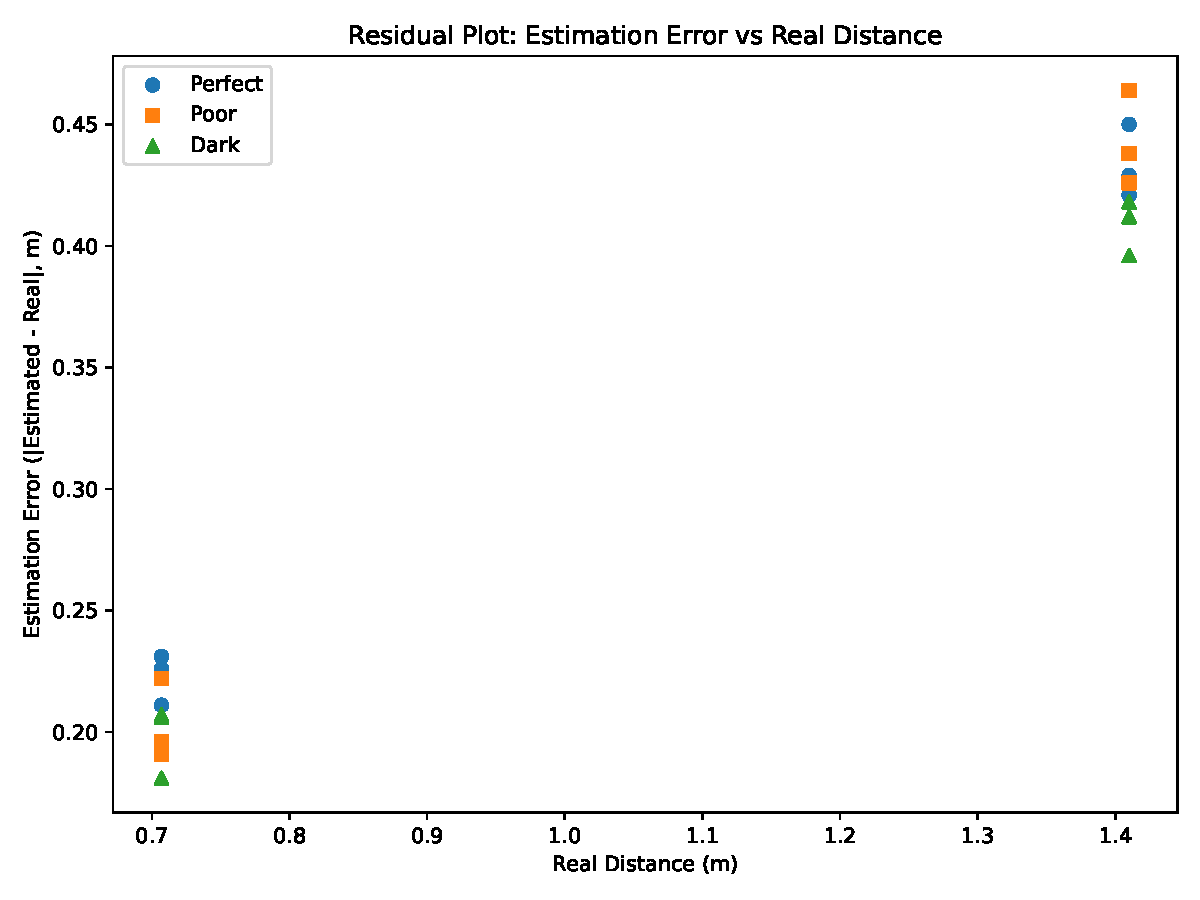
\includegraphics[width=0.9\linewidth]{assets/ch4/distacneerro.pdf}
	\caption{Absolute distance error ($|\mathrm{Estimated} - \mathrm{Real}|$) for each sample under different lighting conditions. Lower values indicate higher distance accuracy.}
	\label{fig:localization_absolute_distance_error}
\end{figure}

\begin{figure}[h!]
	\centering
	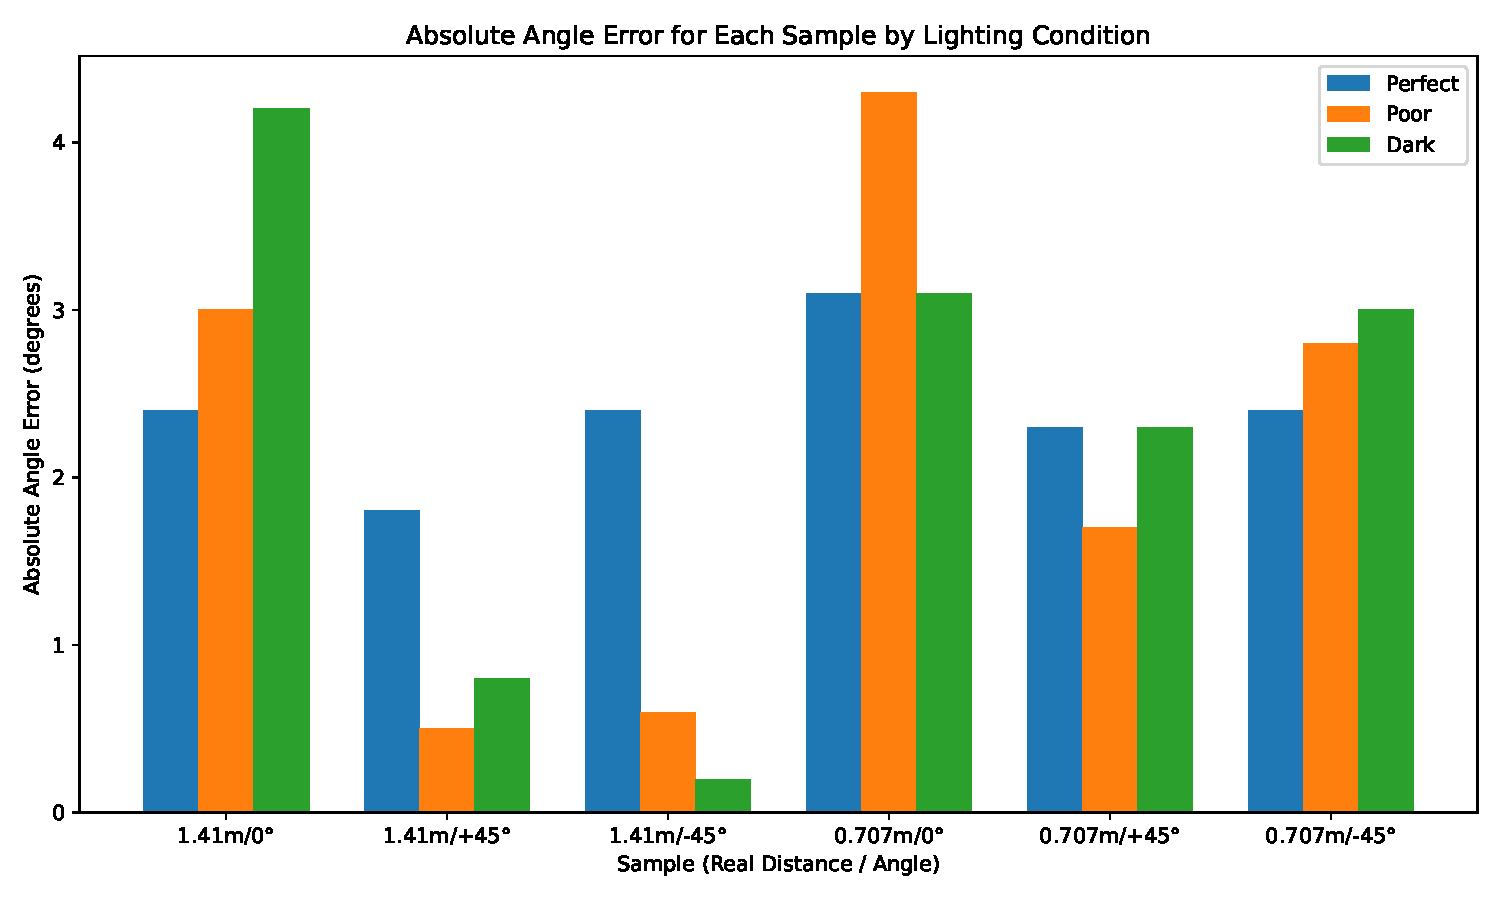
\includegraphics[width=0.9\linewidth]{assets/ch4/angleerro.pdf}
	\caption{Absolute angle error ($|\mathrm{Estimated} - \mathrm{Real}|$) for each sample under different lighting conditions. Lower values indicate higher angular accuracy.}
	\label{fig:localization_absolute_angle_error}
\end{figure}

\subsection{Results Discussion}

As shown in Table~\ref{table:localization_eval}, lighting conditions had negligible impact on accuracy. Notably, the angle estimates were consistently very close to the real values, which is desirable, as precise angles are crucial for user navigation—small deviations could result in significant guidance errors. In contrast, errors in estimated distance are less critical, as the system logic mitigates their effect.

For example, if the estimated distance to a QR code is 2~m while the real value is 2.6~m (a 23\% error), the application adds this to the average distance between milestones (e.g., 3~m), reducing the overall error effect to just 10.7\%. Table~\ref{table:real_estimated_distance_error_effect} illustrates this for typical cases.

\begin{table}[h!]
	\caption{Actual impact of estimated distance errors, assuming an average milestone distance of 3~m.}
	\begin{tabularx}{0.75\textwidth} { 
			| >{\raggedright\arraybackslash}X 
			| >{\centering\arraybackslash}X 
			| >{\centering\arraybackslash}X 
			| >{\raggedleft\arraybackslash}X | }
		\hline
		Estimated Distance & Real Distance & Fake Error Effect & Real Error Effect\\
		\hline
		0.511 m & 0.707 m & 27.722\% & 5.287\%\\
		1.014 m & 1.410 m & 28.085\% & 8.98\%\\
		\hline
	\end{tabularx}
	\label{table:real_estimated_distance_error_effect}
\end{table}
